%% \section{Tutorial}

\subsection{Introduction to Email}

\subsubsection{Messaging}

This chapter is quite different from the rest of this document.
Here we build a foundation for understanding messaging, instead
of focusing on how ZMailer behaves.

This chapter may feel a bit theoretical and abstract, being detached
from practical life.

In reality, however, experience shows that most problems with messaging
are a result of not understanding the underlying messaging model, or of
not respecting said model.

The terminology used here may seem a bit X.400 oriented.
It is, because folks from what was then known as CCITT (now known as ITU-T)
adapted the model originally developed by IFIP.
Of course, CCITT added a lot of things of its own invention (like
ADMDs and PRMDs), that we don't need to bother ourselves with.

Although the terminology comes from X.400, it is in no way restricted to it.
Our presentation here is a generic messaging presentation not restricted
to any type of protocol.

Messaging, as the name says, is all about exchanging messages,
short (or sometimes long) pieces of information.
Messaging is always directional (which means that there is always
a sender and one or more recipients), targeted (the list of recipients
is fixed) and store-and-forward based.

There are a few messaging-like applications in which the message is
broadcast to a wide, unspecified audience.
A prime example of this latter application is Usenet News.
News is not messaging, as it is not targeted.

So what about mailing lists that are linked to News, are they messaging or not?
As long as the message is transported as a mail message, it is messaging.
One of the recipients of the message may well be a Usenet News newsgroup.
Similarly, a sender of a message might be the News system, or the author
who initiated the submission by using News. Messaging is not necessarily
interpersonal.

It is also quite normal for different applications to communicate by using
messaging methods.
A prime example of this would be EDI traffic. It is clearly messaging,
but not interpersonal.



\paragraph{The Messaging Model}

In addition to users, the basic building blocks of messaging are
{\bf User Agents (UAs)} and {\bf Message Transfer Agents (MTAs)}.
User agents are the interface through which a human user interacts with
the messaging system.
On non-interpersonal messaging user agents may be built directly into
applications.
MTAs are used to transport messages from one computer system to another.
An example of a good MTA is ZMailer. 
{\bf Access Units (AUs)} can be used for accessing telematic services,
for example telefax. 
{\bf Message Stores (MSs)} can be used between MTAs and UAs.
They are used for storing messages before and while UAs are used
to access and manipulate them.
{\bf Gateways (GWs)} are used in between two different types
of messaging systems, for example between SMTP and X.400 mail.
Gateways are conceptually made of two MTAs and a UA that interconnects them.

There are two more acronyms worth looking at in the messaging model,
namely {\bf MTS (Message Transport System)} and
{\bf MHS (Message Handling System)}.
MTS is the collection of MTAs (and GWs),
while MHS includes MTS and UA functionality (UAs, MSs and AUs).

{\bf This area will be modified!!!}



A graphical example of the messaging model is shown in figure 
\ref{fig:msgmodl}.
%begin{latexonly}
(Page \pageref{fig:msgmodl}.)
%end{latexonly}
It shows the relationships between different elements of the model.

\begin{figure}[ht]
  \htmlimage{noantialias,transparent}
  \htmlborder{2}
%begin{latexonly}
\fbox{
%end{latexonly}
  \centering\includegraphics[width=\textwidth]{msgmodl.eps}
%begin{latexonly}
}
%end{latexonly}
  \caption{\label{fig:msgmodl}A graphical example of the messaging model.}
\end{figure}


As can be seen, a user may use more than one UA, and a UA can be connected 
to more than one MTA.

Although it is important to understand the relationships between different 
entities in the messaging model, it is even more important to understand the 
nature of a message and the way UAs and MTAs deal with it.

A message consists of a body and headers. In case of messages with more 
than one bodypart (for example some MIME messages) the different body 
parts are all part of the outermost bodypart.

Normally a message looks roughly like this:

\begin{verbatim}
  Headers
        From:   The Manager
        To:     One Bright Employee
        CC:     secretary
        Subject:Salary raise
        Date:   17 May 1997

  Body
        Dear Employee,
        ...
        The Manager
\end{verbatim}

In a more complex case the structure of a message might be something like this:

\begin{verbatim}
  Headers
  Body
        Headers
        Body
                Headers
                Body
                Headers
                Body
        Headers
        Body
\end{verbatim}

As can be seen, there is always just one outermost body that contains 
all other bodyparts. In some cases, for example X.400 the protocol 
seems to violate this by leaving out the outermost bodypart. However, 
even on those cases we must assume, at the abstract level, 
that the outermost bodypart is there.

However, this is not all that there is to the structure of a message. 
When a message is in transit, being handled by MTAs it is put inside 
an envelope, just like a normal letter is inside an envelope while 
the postal service is carrying it. Just like the postal service is not 
permitted to look inside the envelope, neither are MTAs permitted 
to look inside. Whenever there is a need to look inside the envelope, 
it is always a UA function, and done on behalf, and on the authority of, a UA.

There are some violations of this. When using the SMTP protocol, the 
{\tt Received:} lines are put in the headers by MTAs. This is bad 
engineering, but as the process of adding a new header line is fairly 
straightforward, it doesn't cause too much pain. In some cases MTAs 
modify the header even more, and sometimes they even mess with the body. 
This is a sure recipe for trouble.



Graphically, the way a message should be dealt with is shown 
in figure
%begin{latexonly}
 \ref{fig:msgrout}, page \pageref{fig:msgrout}.
%end{latexonly}
\begin{figure}[ht]
  \htmlimage{noantialias,transparent}
  \htmlborder{2}
  \centering
%begin{latexonly}
\fbox{
%end{latexonly}
  \includegraphics[width=\textwidth]{msgrout.eps}
%begin{latexonly}
}
%end{latexonly}
  \caption{\label{fig:msgrout}How a message should be handled.}
\end{figure}

The user creates the message with the help of a UA. How the interaction 
is arranged is a local matter. Once the message has been prepared, 
it is passed to a nearby MTA together with necessary envelope 
information and put into an envelope. The MTA puts its stamp on 
the envelope to show that it has received the message. The first 
MTA passes the message to the second MTA. The second MTA puts its 
stamp to the message and passes it to the third MTA, and so on. 
The final MTA passes the message to a UA, and the envelope is removed.

There are at least three ways to pass the message from an MTA to a UA. 
The message may be pushed to a (running) UA, a UA may pull it from an MTA, 
or an MTA may pass the message to an MS from which a UA will receive it at 
a convenient time.

The normal UNIX way of delivering mail ({\tt /usr/spool/mail/user}) can be 
seen as any of the above three mechanisms, but should normally be seen as a 
UA pulling a message. The reason for this confusion is with the de-facto SMTP 
standard MTA, Sendmail. Although Sendmail is in many ways a very clever 
piece of software, it is also the reason for many problems, as it has 
blurred the line between MTA and UA. Sendmail is clearly an MTA, but 
it also performs many of the UA level functions, like handling of 
{\tt .forward} files. This behaviour has become the de-facto standard 
way for UNIX MTAs to behave, making it necessary for any MTA, including
ZMailer, to behave the same way.



\paragraph{Routing And Delivering Messages}



As MTAs only deal with envelopes, all routing and delivery decisions have to be
based on information available on the envelope. It follows from this that 
the envelope and headers may contain conflicting information. This is normal, 
and is not a cause for worry.

MTAs may, and often do modify addresses present in the envelope. This might 
include changing addresses to a format more suitable for mail delivery and 
alias expansion.

It is important to make a distinction between aliasing and forwarding mail. 
Aliasing is an MTA function, in which an MTA effectively knows that to reach 
a seemingly local user, mail should be sent to a different address. 
To accomplish this, the MTA changes the recipient information on the envelope. 
Forwarding is a UA function. When forwarding, the mail message is received 
by the original, intended recipient, and re-sent to another address. Although 
forwarding is a UA function, it doesn't have to result in a change to body or 
headers, but on the envelope, both sender and recipient should be changed. 
Sendmail bluntly violates this, and makes most other MTAs violate it as well.

Most mailing lists today are just alias expansions, on which one recipient 
address on the envelope is replaced with multiple addresses. In many cases 
this is a reasonable approach. However, all major mailing lists should be 
set up as a UA function. This involves changing not only the recipient 
address but also the sender address in the envelope. In this way, 
undeliverable messages are sent to the owner of the list, who can deal 
with the problem, and not to the sender of the message, who can do nothing 
to remedy the situation.

Error messages must be sent to the envelope sender address, as this is a 
MTA function. If a header like {\tt Errors-to:} is being used, it implies 
that envelope sender should be sent to the one in the {\tt Errors-to:} header.

Replies to messages should be sent to header addresses, because replying is 
a UA function.




\subsection{ZMailer's Features and Facilities}




\subsubsection{Introduction}

ZMailer is a mailer subsystem for the UNIX operating system.
It is in charge of handling all mail messages that are created
on a system, from their creation until final disposition locally
or by transfer to another system.

As such, the mailer subsystem (the Message Transfer Agent) must
interface to local mail reading and composing programs (User Agents),
to the various transport methods that can be used to reach other mailers,
and to a variety of databases describing the mailer's environment.

ZMailer provides this functionality in a package and with a philosophy
that has benefited from experiences with earlier mailers.

ZMailer provides a capable, robust, efficient subsystem to do the job,
which will excel in demanding environments, but is simple enough to
fit easily everywhere.


\subsubsection{Design Summary}

ZMailer is a multi-process mailer, using two daemon processes to manipulate
messages.  One of these processes is a router, and makes all decisions
about what should happen to a message.  The other daemon is a message queue
manager, used to schedule delivery of messages.  The Router uses a
configuration file that closely follows Bourne shell script syntax and
semantics, with minimal magic.  Message files are moved around in a series
of directories, and the Scheduler and its Transport Agents run off of
control files created by the Router.

The Router will process messages one at a time, as it finds them in a
directory where User Agents submit their outgoing messages.  Envelope and
Message Header information is all kept in the same message file along with
the message body, and this file is never modified by any ZMailer program.
After parsing the envelope and RFC822 header information, the Router
validates the information extracted, and calls functions defined in the
configuration file to decide exactly how to deliver the message and how to
transform the embedded addresses.  The algorithms that do this are easily
reconfigurable, since the control flow and address manipulation is
specified by familiar shell script statements.  When the Router is
finished, it will produce a message control file for use by the delivery
processing stage of ZMailer, and move the original message file to another
location.

Once the Router has decided what to do with each of the addresses in a
message, the Scheduler builds a summary of this information by reading the
control file created by the Router.  This knowledge is merged with a data
structure it maintains that stores which messages are supposed to be sent
where, and how.  According to a pre-arranged agenda, the Scheduler will
execute delivery programs to properly move the message envelope, header,
and body, to the immediate destination.  These delivery programs are called
Transport Agents, and communicate with the Scheduler using a simple
protocol that tells them which messages to process and returns status
reports to the Scheduler.  The Scheduler also manages status reports,
taking appropriate action on delivery errors and when all delivery
instructions for a message have been processed.

There are several standard Transport Agents included with the ZMailer
distribution.  The collection currently includes a local delivery program,
an SMTP client implementation, and a Transport Agent that can run
Sendmail-compatible delivery programs.

A separate utility allows querying the Scheduler for the state of its mail
queues.  For existing Sendmail installations, a replacement program is
included that simulates most of the Sendmail functionality in the ZMailer
environment.  This allows ZMailer to replace a Sendmail installation
without requiring changes in standard User Agents.


\begin{figure}[ht]
  \htmlimage{noantialias,transparent}
  \htmlborder{2}
  \centering
%begin{latexonly}
\fbox{
%end{latexonly}
  \includegraphics[width=\textwidth]{zmdirs.eps}
%begin{latexonly}
}
%end{latexonly}
  \caption{\label{fig:zmdirs}Directories that ZMailer uses for message processing}
\end{figure}


\subsection{Running ZMailer}

ZMailer is fairly simple to run, once the setups are completed
it can be left to run on its own with very little supervision.

Things that might need supervision are things like:
\begin{itemize}
\item Timely cycling of log files, which otherwise will grow until
they fill all of the available disk space  (One need not log
everything possible, about the only thing this system does not
allow you to log is the message body content.)
\item Keeping watchful eye on  {\tt \$POSTOFFICE/freezer/}, and 
{\tt \$POSTOFFICE/postman/}
directories.  Former for processing SPAM email, latter for
pathological problem cases.  (More at  3.3.4)
\end{itemize}

We look closer into these issues at latter parts of this document,
but now it is sufficient to tell, that the principal tool for active
monitoring of the system health is command:
\begin{verbatim}
  mailq -ss
\end{verbatim}

which does tell, if router, or scheduler are up and about, or not,
and also does tell about the sizes of the different sub-spools.

The general management interface for starting and stopping different
subsystems is command
\begin{verbatim}
  zmailer
\end{verbatim}

which the system installs into {\tt \$MAILBIN/} directory, and which command usually needs a symlink to itself from some more common location for
administrative convenience
( {\tt /usr/sbin/zmailer --> \$MAILBIN/zmailer} )
so that the administrator does not need to add  {\tt \$MAILBIN/}  directory
into his or her {\tt PATH}.   On overall, it is intention that not even 
admin
user should need to run directly the programs at the {\tt \$MAILBIN/} directory.

Basically the administration is as follows:
\begin{itemize}
\item At system startup (to start all subsystems):
\begin{verbatim}
  zmailer
\end{verbatim}
\item At system shutdown (to kill all subsystems):
\begin{verbatim}
  zmailer kill
\end{verbatim}
\end{itemize}

There is also a way to make sure the system will not let the ZMailer
to start at the system startup, because you have some massive work
going on, and the system is not in condition to accept email for a while: 
\begin{verbatim}
  zmailer freeze
\end{verbatim}

and the antidote for the ``freeze'' is, naturally:
\begin{verbatim}
  zmailer thaw
\end{verbatim}

Normal operations can not be started at ``frozen'' system without ``thawing'' it at first.

The user-visible component of the ZMailer is (for de-facto interface)
\begin{verbatim}
  /usr/lib/sendmail
\end{verbatim}

(a.k.a.) {\tt /usr/sbin/sendmail}
which is ``simple'' message submission program that mimics sendmail
commands behaviour, but of course many details of sendmail are
not really implemented at all, mostly because they do not have
equivalents in the ZMailer system.

There are also functional equivalents (or near equivalents) of
other sendmail/system utilities:  {\em mailq\/}, {\em newaliases\/}, {\em vacation\/}




\subsection{Comparison With Other Popular MTA's}

{\bf Sendmail}, in the right hands, can be quite a flexible tool to translate
between the different conventions of various networks.  Unfortunately this
is accomplished by programming in an unfamiliar production language
containing many magic features.  The learning time for doing this is very
long, the effort involved is that of learning a completely new language and
environment. Moreover, Sendmail has all major components built into a
single large program. Both of these design decisions have been acknowledged
as mistakes by the author of Sendmail.  Its major shortcoming in comparison
to the MMDF mailer is its primitive database facility and lack of caching.

{\bf MMDF} is a comprehensive mail environment, including its own mail
composition program and of course a mailer.  There are too many parts to it
(as can be said, it is a system, not a subsystem), and the address
manipulation is only sufficient for a relatively homogenous environment. It
does have reasonable database facilities and caching, as opposed to
Sendmail, and the concept of Channels.  However, knowledge about address
semantics is distributed in several programs instead of being centralized.
{\bf PMDF} is a smaller version of MMDF with correspondingly reduced features and
flexibility.

{\bf Upas} is a curious approach to the problem. It lets the user do half the
work of message routing, in a manner similar to PMDF on VMS systems. It is
entirely concerned with the message envelope, and leaves all message header
munging to auxiliary programs if appropriate. In fairness one should note
this mailer was developed in an environment where most message headers were
scorned, thus making this a reasonable approach (``optimize the normal
case''). The Eighth Edition Upas had no database capability at all, but it
did exhibit one useful characteristic: the routing decisions are made by
passing the recipient envelope address through a set of regular
expressions. This production rule approach is similar to what Sendmail
does, but uses a more familiar mechanism and environment.

The final, and most recently developed, mailer worth mentioning here is
{\bf Smail3.0}.
It is intended as a program capable of replacing Sendmail in many
situations. To a large extent it succeeds as this, and there are some nice
ideas involved as well. Its two major drawbacks are that it is not as easy
to adapt to local needs as Sendmail is (compiled instead of interpreted
rules and algorithms), and retaining Sendmail's single-program design.  It
addresses database and caching issues, and seems generally like a nicer
design in many respects, a bit like PMDF's configuration options in a
Sendmail package.

Until the recent increase in the demand for inter-network mail gatewaying,
Sendmail's flexibility had quite adequately served to implement a gateway
function between selected networks.  With increased variety of the normal
address syntax and mail capabilities of connected networks, and more complex
kinds of routing decisions becoming necessary, the existing mailers have
been showing their age and their limits.  ZMailer is intended to give the
mail administrator a software tool that fits the times.
